\documentclass[11pt,a4paper]{article}

% ── Packages ──────────────────────────────────────────────────────────
\usepackage[utf8]{inputenc}
\usepackage[T1]{fontenc}
\usepackage{lmodern}
\usepackage[margin=1in]{geometry}
\usepackage{hyperref}
\usepackage{graphicx}
\usepackage{xcolor}
\usepackage{listings}
\usepackage{booktabs}
\usepackage{longtable}
\usepackage{array}
\usepackage{enumitem}
\usepackage{tikz}
\usetikzlibrary{shapes.geometric, arrows.meta, positioning, fit, calc, decorations.pathreplacing}
\usepackage{float}
\usepackage{fancyhdr}
\usepackage{tocloft}
\usepackage{titlesec}
\usepackage{amsmath}
\usepackage{textcomp}
\usepackage{parskip}

% ── Colors ────────────────────────────────────────────────────────────
\definecolor{primary}{HTML}{2563EB}
\definecolor{secondary}{HTML}{64748B}
\definecolor{success}{HTML}{16A34A}
\definecolor{warning}{HTML}{D97706}
\definecolor{danger}{HTML}{DC2626}
\definecolor{codebg}{HTML}{F8FAFC}
\definecolor{codeframe}{HTML}{E2E8F0}

% ── Listings ──────────────────────────────────────────────────────────
\lstdefinestyle{python}{
  language=Python,
  basicstyle=\ttfamily\small,
  keywordstyle=\color{primary}\bfseries,
  stringstyle=\color{success},
  commentstyle=\color{secondary}\itshape,
  backgroundcolor=\color{codebg},
  frame=single,
  rulecolor=\color{codeframe},
  breaklines=true,
  showstringspaces=false,
  tabsize=4,
  numbers=left,
  numberstyle=\tiny\color{secondary},
}
\lstdefinestyle{typescript}{
  language=Java,
  basicstyle=\ttfamily\small,
  keywordstyle=\color{primary}\bfseries,
  stringstyle=\color{success},
  commentstyle=\color{secondary}\itshape,
  backgroundcolor=\color{codebg},
  frame=single,
  rulecolor=\color{codeframe},
  breaklines=true,
  showstringspaces=false,
  tabsize=2,
  numbers=left,
  numberstyle=\tiny\color{secondary},
  morekeywords={interface,type,export,const,let,async,await,import,from,extends,implements,readonly},
}

% ── Header/Footer ────────────────────────────────────────────────────
\pagestyle{fancy}
\fancyhf{}
\fancyhead[L]{\small\textcolor{secondary}{ReviewPyPer React -- Technical Report}}
\fancyhead[R]{\small\textcolor{secondary}{\today}}
\fancyfoot[C]{\thepage}
\renewcommand{\headrulewidth}{0.4pt}

% ── Title config ─────────────────────────────────────────────────────
\titleformat{\section}{\Large\bfseries\color{primary}}{\thesection}{1em}{}
\titleformat{\subsection}{\large\bfseries\color{primary!80!black}}{\thesubsection}{1em}{}
\titleformat{\subsubsection}{\normalsize\bfseries\color{primary!60!black}}{\thesubsubsection}{1em}{}

\hypersetup{
  colorlinks=true,
  linkcolor=primary,
  urlcolor=primary,
  citecolor=primary,
}

% ══════════════════════════════════════════════════════════════════════
\begin{document}

% ── Title Page ────────────────────────────────────────────────────────
\begin{titlepage}
\centering
\vspace*{2cm}
{\Huge\bfseries\color{primary} ReviewPyPer React\\[0.3cm]}
{\Large\color{secondary} Full-Stack Systematic Review Platform\\[0.5cm]}
{\large Technical Architecture \& API Documentation\\[2cm]}


\begin{tikzpicture}
\draw[primary, line width=2pt] (0,0) -- (12,0);
\end{tikzpicture}

\vspace{1.5cm}
{\large
\begin{tabular}{rl}
\textbf{Version:} & 2.0 (React Rewrite) \\
\textbf{Date:} & \today \\
\textbf{Stack:} & React + TypeScript + Tailwind CSS / FastAPI + Python \\
\textbf{Original:} & ReviewPyPer (Streamlit) by Calvin Whow \\
\end{tabular}
}

\vfill
{\small Comprehensive documentation of every module, function, endpoint, component, and data flow.}
\end{titlepage}

% ── Table of Contents ────────────────────────────────────────────────
\tableofcontents
\newpage

% ══════════════════════════════════════════════════════════════════════
\section{Executive Summary}
% ══════════════════════════════════════════════════════════════════════

ReviewPyPer React is a full-stack rewrite of the ReviewPyPer systematic review platform. The original application, built with Streamlit, has been decomposed into a \textbf{React + TypeScript frontend} and a \textbf{FastAPI backend}, with the original Python core modules retained as the business logic layer.

The platform automates the systematic review workflow following \textbf{PRISMA 2020 guidelines}, leveraging Large Language Models (OpenAI GPT and Anthropic Claude) for:

\begin{itemize}[nosep]
  \item PICO-based screening criteria generation
  \item Title/abstract and full-text study screening
  \item Structured data extraction from PDFs
  \item Risk of Bias assessment using validated tools (RoB~2, ROBINS-I, QUADAS-2, Newcastle-Ottawa, JBI)
  \item Multi-database search strategy generation and translation
\end{itemize}

\subsection{Architecture Overview}

\begin{figure}[H]
\centering
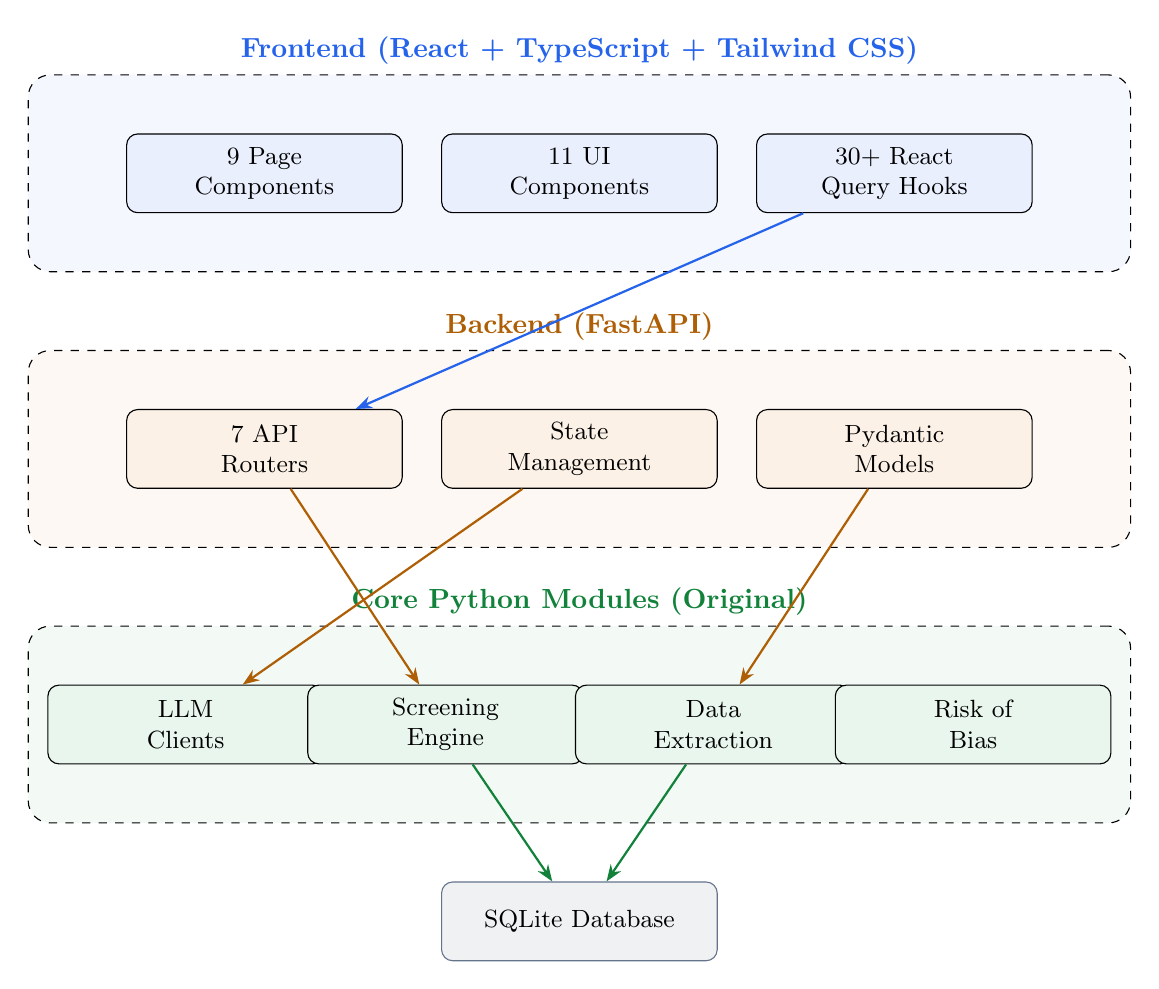
\begin{tikzpicture}[
  box/.style={draw, rounded corners=4pt, minimum width=3.5cm, minimum height=1cm, align=center, font=\small},
  layer/.style={draw, dashed, rounded corners=8pt, inner sep=10pt, fill=#1!5},
  arr/.style={-{Stealth[length=6pt]}, thick},
]
% Frontend layer
\node[layer=primary, minimum width=14cm, minimum height=2.5cm, label={[font=\bfseries\color{primary}]above:Frontend (React + TypeScript + Tailwind CSS)}] (fe) at (0,5) {};
\node[box, fill=primary!10] (pages) at (-4,5) {9 Page\\Components};
\node[box, fill=primary!10] (ui) at (0,5) {11 UI\\Components};
\node[box, fill=primary!10] (hooks) at (4,5) {30+ React\\Query Hooks};

% API layer
\node[layer=warning, minimum width=14cm, minimum height=2.5cm, label={[font=\bfseries\color{warning!80!black}]above:Backend (FastAPI)}] (be) at (0,1.5) {};
\node[box, fill=warning!10] (routers) at (-4,1.5) {7 API\\Routers};
\node[box, fill=warning!10] (state) at (0,1.5) {State\\Management};
\node[box, fill=warning!10] (models) at (4,1.5) {Pydantic\\Models};

% Core layer
\node[layer=success, minimum width=14cm, minimum height=2.5cm, label={[font=\bfseries\color{success!80!black}]above:Core Python Modules (Original)}] (core) at (0,-2) {};
\node[box, fill=success!10] (llm) at (-5,-2) {LLM\\Clients};
\node[box, fill=success!10] (screening) at (-1.7,-2) {Screening\\Engine};
\node[box, fill=success!10] (extraction) at (1.7,-2) {Data\\Extraction};
\node[box, fill=success!10] (rob) at (5,-2) {Risk of\\Bias};

% Storage
\node[box, fill=secondary!10, draw=secondary] (db) at (0,-4.5) {SQLite Database};

% Arrows
\draw[arr, primary] (hooks) -- (routers);
\draw[arr, warning!80!black] (routers) -- (screening);
\draw[arr, warning!80!black] (state) -- (llm);
\draw[arr, warning!80!black] (models) -- (extraction);
\draw[arr, success!80!black] (screening) -- (db);
\draw[arr, success!80!black] (extraction) -- (db);

\end{tikzpicture}
\caption{Three-layer architecture: Frontend, Backend API, and Core Python modules.}
\end{figure}

% ══════════════════════════════════════════════════════════════════════
\section{System Architecture}
% ══════════════════════════════════════════════════════════════════════

\subsection{Directory Structure}

\begin{lstlisting}[style=python, title=Project Layout]
reviewpyper-react/
|-- frontend/                  # React + Vite + Tailwind
|   |-- src/
|   |   |-- types/index.ts     # 15 TypeScript interfaces
|   |   |-- services/api.ts    # Axios API client
|   |   |-- hooks/useApi.ts    # 30+ React Query hooks
|   |   |-- components/
|   |   |   |-- layout/        # AppLayout, Sidebar
|   |   |   |-- ui/            # 11 reusable UI components
|   |   |   |-- PrismaFlow.tsx # PRISMA 2020 diagram
|   |   |-- pages/             # 9 workflow step pages
|   |   |-- App.tsx            # Router + providers
|   |   |-- main.tsx           # Entry point
|   |-- vite.config.ts
|   |-- package.json
|
|-- backend/                   # FastAPI
|   |-- main.py                # App entry + CORS + routers
|   |-- requirements.txt
|   |-- services/
|   |   |-- state.py           # Global state management
|   |-- routers/               # 7 API router modules
|       |-- projects.py
|       |-- llm.py
|       |-- screening.py
|       |-- extraction.py
|       |-- risk_of_bias.py
|       |-- search_strategy.py
|       |-- export.py
|
|-- docs/                      # This report
\end{lstlisting}

\subsection{Technology Stack}

\begin{table}[H]
\centering
\begin{tabular}{lll}
\toprule
\textbf{Layer} & \textbf{Technology} & \textbf{Purpose} \\
\midrule
Frontend Framework & React 19 + TypeScript & UI rendering \\
Build Tool & Vite 6 & Development server + bundler \\
Styling & Tailwind CSS v4 & Utility-first CSS \\
State/Data & TanStack React Query & Server state management \\
HTTP Client & Axios & API communication \\
Icons & Lucide React & SVG icon library \\
Routing & React Router v7 & Client-side routing \\
\midrule
Backend Framework & FastAPI & REST API server \\
ASGI Server & Uvicorn & Production server \\
Validation & Pydantic v2 & Request/response models \\
Database & SQLite & Project data persistence \\
\midrule
LLM Providers & OpenAI SDK, Anthropic SDK & AI capabilities \\
PDF Processing & PyPDF2, Tesseract OCR & Text extraction \\
File Parsing & Custom parsers & CSV, RIS, NBIB, BibTeX, EndNote \\
\bottomrule
\end{tabular}
\caption{Complete technology stack.}
\end{table}

% ══════════════════════════════════════════════════════════════════════
\section{Call Graph: Complete System Flow}
% ══════════════════════════════════════════════════════════════════════

\subsection{End-to-End Workflow Call Graph}

\begin{figure}[H]
\centering
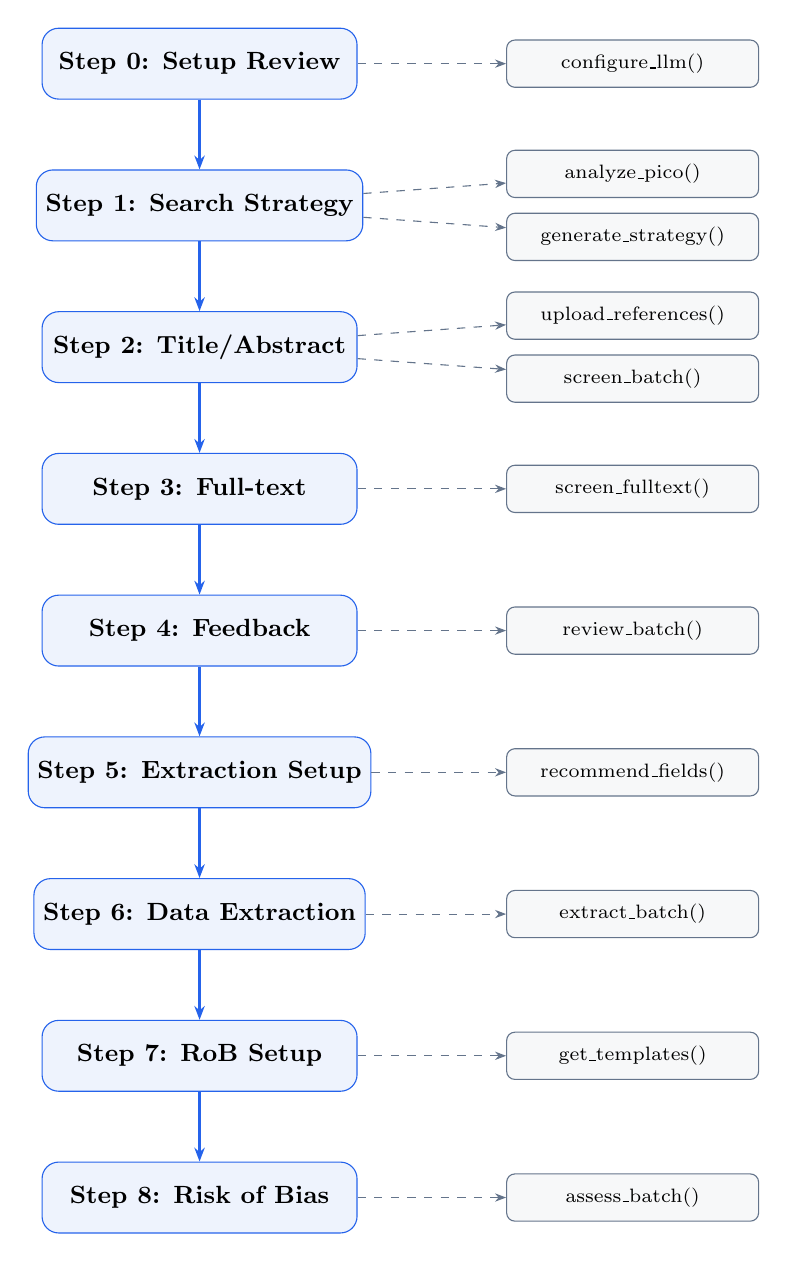
\begin{tikzpicture}[
  wfstep/.style={draw=primary, fill=primary!8, rounded corners=6pt, minimum width=4cm, minimum height=0.9cm, align=center, font=\small\bfseries},
  detail/.style={draw=secondary, fill=secondary!5, rounded corners=3pt, minimum width=3.2cm, minimum height=0.6cm, align=center, font=\scriptsize},
  arr/.style={-{Stealth[length=5pt]}, thick, primary},
  darr/.style={-{Stealth[length=4pt]}, secondary, dashed},
]

\node[wfstep] (s0) at (0,0) {Step 0: Setup Review};
\node[wfstep] (s1) at (0,-1.8) {Step 1: Search Strategy};
\node[wfstep] (s2) at (0,-3.6) {Step 2: Title/Abstract};
\node[wfstep] (s3) at (0,-5.4) {Step 3: Full-text};
\node[wfstep] (s4) at (0,-7.2) {Step 4: Feedback};
\node[wfstep] (s5) at (0,-9.0) {Step 5: Extraction Setup};
\node[wfstep] (s6) at (0,-10.8) {Step 6: Data Extraction};
\node[wfstep] (s7) at (0,-12.6) {Step 7: RoB Setup};
\node[wfstep] (s8) at (0,-14.4) {Step 8: Risk of Bias};

% Right side details
\node[detail] (d0) at (5.5,0) {configure\_llm()};
\node[detail] (d1a) at (5.5,-1.4) {analyze\_pico()};
\node[detail] (d1b) at (5.5,-2.2) {generate\_strategy()};
\node[detail] (d2a) at (5.5,-3.2) {upload\_references()};
\node[detail] (d2b) at (5.5,-4.0) {screen\_batch()};
\node[detail] (d3) at (5.5,-5.4) {screen\_fulltext()};
\node[detail] (d4) at (5.5,-7.2) {review\_batch()};
\node[detail] (d5) at (5.5,-9.0) {recommend\_fields()};
\node[detail] (d6) at (5.5,-10.8) {extract\_batch()};
\node[detail] (d7) at (5.5,-12.6) {get\_templates()};
\node[detail] (d8) at (5.5,-14.4) {assess\_batch()};

\foreach \i/\j in {s0/s1, s1/s2, s2/s3, s3/s4, s4/s5, s5/s6, s6/s7, s7/s8}
  \draw[arr] (\i) -- (\j);

\foreach \i/\j in {s0/d0, s1/d1a, s1/d1b, s2/d2a, s2/d2b, s3/d3, s4/d4, s5/d5, s6/d6, s7/d7, s8/d8}
  \draw[darr] (\i) -- (\j);

\end{tikzpicture}
\caption{9-step systematic review workflow with core function calls.}
\end{figure}

\subsection{Screening Pipeline Call Graph}

\begin{figure}[H]
\centering
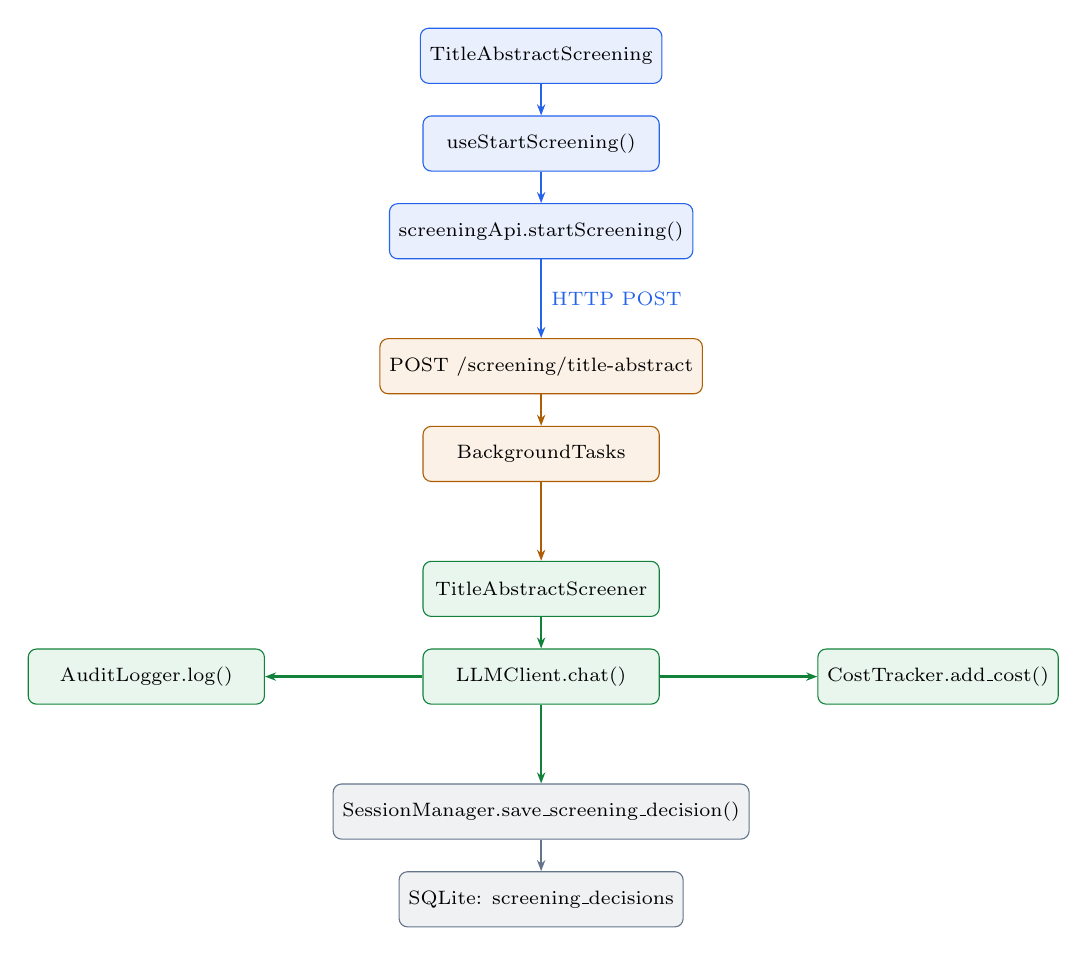
\begin{tikzpicture}[
  node distance=0.4cm and 1.5cm,
  box/.style={draw, rounded corners=3pt, minimum width=3cm, minimum height=0.7cm, align=center, font=\scriptsize},
  fe/.style={box, fill=primary!10, draw=primary},
  be/.style={box, fill=warning!10, draw=warning!80!black},
  core/.style={box, fill=success!10, draw=success!80!black},
  db/.style={box, fill=secondary!10, draw=secondary},
  arr/.style={-{Stealth[length=4pt]}, thick},
]

% Frontend
\node[fe] (page) {TitleAbstractScreening};
\node[fe, below=of page] (hook) {useStartScreening()};
\node[fe, below=of hook] (api) {screeningApi.startScreening()};

% Backend
\node[be, below=1cm of api] (router) {POST /screening/title-abstract};
\node[be, below=of router] (bg) {BackgroundTasks};

% Core
\node[core, below=1cm of bg] (screener) {TitleAbstractScreener};
\node[core, below=of screener] (llmcall) {LLMClient.chat()};
\node[core, right=2cm of llmcall] (cost) {CostTracker.add\_cost()};
\node[core, left=2cm of llmcall] (audit) {AuditLogger.log()};

% DB
\node[db, below=1cm of llmcall] (save) {SessionManager.save\_screening\_decision()};
\node[db, below=of save] (sqlite) {SQLite: screening\_decisions};

% Arrows
\draw[arr, primary] (page) -- (hook);
\draw[arr, primary] (hook) -- (api);
\draw[arr, primary] (api) -- node[right, font=\scriptsize] {HTTP POST} (router);
\draw[arr, warning!80!black] (router) -- (bg);
\draw[arr, warning!80!black] (bg) -- (screener);
\draw[arr, success!80!black] (screener) -- (llmcall);
\draw[arr, success!80!black] (llmcall) -- (cost);
\draw[arr, success!80!black] (llmcall) -- (audit);
\draw[arr, success!80!black] (llmcall) -- (save);
\draw[arr, secondary] (save) -- (sqlite);

\end{tikzpicture}
\caption{Title/abstract screening call graph from UI click to database persistence.}
\end{figure}

\subsection{LLM Client Call Graph}

\begin{figure}[H]
\centering
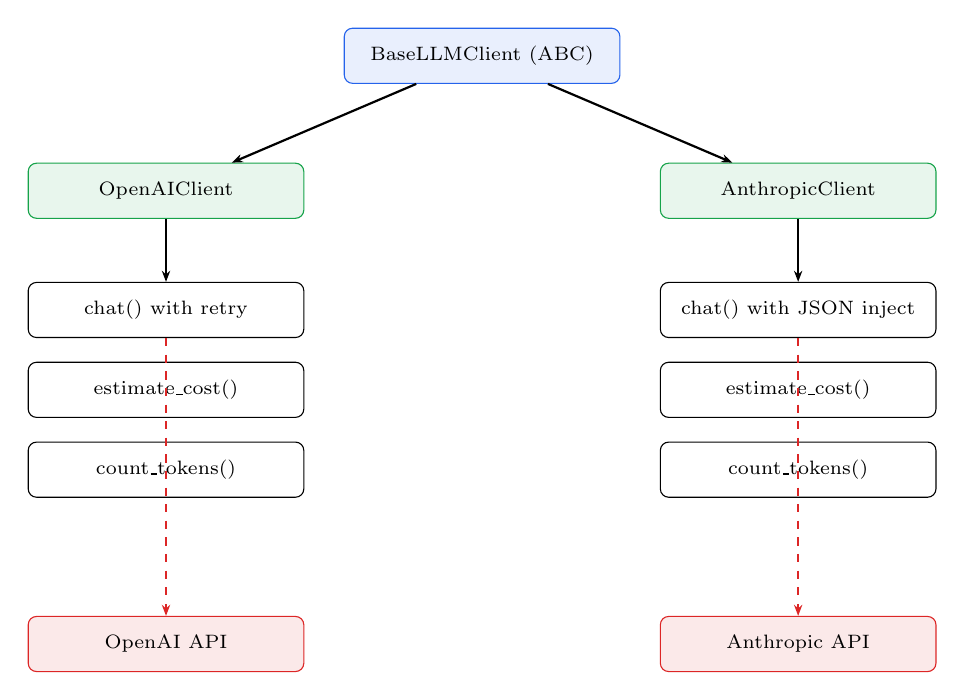
\begin{tikzpicture}[
  node distance=0.5cm and 2cm,
  box/.style={draw, rounded corners=3pt, minimum width=3.5cm, minimum height=0.7cm, align=center, font=\scriptsize},
  abs/.style={box, fill=primary!10, draw=primary},
  impl/.style={box, fill=success!10, draw=success},
  ext/.style={box, fill=danger!10, draw=danger},
  arr/.style={-{Stealth[length=4pt]}, thick},
]

\node[abs] (base) {BaseLLMClient (ABC)};
\node[impl, below left=1cm and 0.5cm of base] (oai) {OpenAIClient};
\node[impl, below right=1cm and 0.5cm of base] (anth) {AnthropicClient};

\node[box, below=0.8cm of oai] (oai_chat) {chat() with retry};
\node[box, below=0.3cm of oai_chat] (oai_cost) {estimate\_cost()};
\node[box, below=0.3cm of oai_cost] (oai_tok) {count\_tokens()};

\node[box, below=0.8cm of anth] (anth_chat) {chat() with JSON inject};
\node[box, below=0.3cm of anth_chat] (anth_cost) {estimate\_cost()};
\node[box, below=0.3cm of anth_cost] (anth_tok) {count\_tokens()};

\node[ext, below=1.5cm of oai_tok] (openai_api) {OpenAI API};
\node[ext, below=1.5cm of anth_tok] (claude_api) {Anthropic API};

\draw[arr] (base) -- (oai);
\draw[arr] (base) -- (anth);
\draw[arr] (oai) -- (oai_chat);
\draw[arr] (anth) -- (anth_chat);
\draw[arr, dashed, danger] (oai_chat) -- (openai_api);
\draw[arr, dashed, danger] (anth_chat) -- (claude_api);

\end{tikzpicture}
\caption{LLM client inheritance and external API calls.}
\end{figure}

% ══════════════════════════════════════════════════════════════════════
\section{Core Python Modules (Original)}
% ══════════════════════════════════════════════════════════════════════

The core Python modules provide all business logic. The FastAPI backend wraps these modules with HTTP endpoints.

\subsection{LLM Module (\texttt{core/llm/})}

\subsubsection{BaseLLMClient (base\_client.py)}

Abstract base class defining the LLM provider interface.

\begin{table}[H]
\centering
\begin{tabular}{p{4cm}p{4cm}p{5cm}}
\toprule
\textbf{Method} & \textbf{Signature} & \textbf{Description} \\
\midrule
\texttt{\_\_init\_\_} & \texttt{(api\_key, model)} & Initialize with credentials \\
\texttt{chat} & \texttt{(messages, temperature, max\_tokens, json\_mode) $\to$ LLMResponse} & Send chat request (abstract) \\
\texttt{estimate\_cost} & \texttt{(input\_tokens, output\_tokens) $\to$ float} & Estimate USD cost (abstract) \\
\texttt{count\_tokens} & \texttt{(text) $\to$ int} & Count tokens in text (abstract) \\
\texttt{provider\_name} & property $\to$ \texttt{str} & Provider identifier (abstract) \\
\texttt{supported\_models} & property $\to$ \texttt{list[str]} & Available models (abstract) \\
\bottomrule
\end{tabular}
\caption{BaseLLMClient abstract interface.}
\end{table}

\textbf{LLMResponse} dataclass: \texttt{content: str}, \texttt{input\_tokens: int}, \texttt{output\_tokens: int}, \texttt{cost: float}.

\subsubsection{OpenAIClient (openai\_client.py)}

Implements \texttt{BaseLLMClient} for OpenAI GPT models.

\begin{itemize}[nosep]
  \item \textbf{Default model:} \texttt{gpt-4o}
  \item \textbf{Supported models:} GPT-5.2-pro, GPT-5.2, GPT-5, GPT-5-mini, GPT-5-nano, GPT-4.1, GPT-4o, GPT-4o-mini, GPT-4-turbo, GPT-3.5-turbo
  \item \textbf{Retry logic:} Auto-retry on rate limit (429) and server errors (5xx), up to 5 retries with exponential backoff
  \item \textbf{Rate limit parsing:} Extracts wait time from error message (``try again in Xms/Xs'')
  \item \textbf{Token counting:} Uses \texttt{tiktoken} library with fallback to character-based estimation
  \item \textbf{JSON mode:} Supported via \texttt{response\_format=\{"type": "json\_object"\}}
  \item \textbf{chat\_safe():} Graceful error handling that returns a safe fallback on failure
\end{itemize}

\begin{table}[H]
\centering\small
\begin{tabular}{lrr}
\toprule
\textbf{Model} & \textbf{Input (\$/1M)} & \textbf{Output (\$/1M)} \\
\midrule
gpt-5.2-pro & \$15.00 & \$60.00 \\
gpt-5 & \$10.00 & \$30.00 \\
gpt-4o & \$5.00 & \$15.00 \\
gpt-4o-mini & \$0.15 & \$0.60 \\
gpt-3.5-turbo & \$0.50 & \$1.50 \\
\bottomrule
\end{tabular}
\caption{OpenAI model pricing (per 1M tokens).}
\end{table}

\subsubsection{AnthropicClient (anthropic\_client.py)}

Implements \texttt{BaseLLMClient} for Anthropic Claude models.

\begin{itemize}[nosep]
  \item \textbf{Default model:} \texttt{claude-sonnet-4-20250514}
  \item \textbf{Supported models:} Claude Sonnet 4, Claude Opus 4, Claude 3.7 Sonnet, Claude 3.5 Sonnet/Haiku, Claude 3 series
  \item \textbf{Token counting:} Character-based approximation (\texttt{CHARS\_PER\_TOKEN = 4.0})
  \item \textbf{JSON mode:} Injected via system prompt (``Respond only with valid JSON'')
  \item \textbf{System messages:} Extracted from message list and passed as separate \texttt{system} parameter
\end{itemize}

\begin{table}[H]
\centering\small
\begin{tabular}{lrr}
\toprule
\textbf{Model} & \textbf{Input (\$/1M)} & \textbf{Output (\$/1M)} \\
\midrule
claude-opus-4 & \$15.00 & \$75.00 \\
claude-sonnet-4 & \$3.00 & \$15.00 \\
claude-3.5-haiku & \$0.80 & \$4.00 \\
\bottomrule
\end{tabular}
\caption{Anthropic model pricing (per 1M tokens).}
\end{table}

\subsubsection{Prompt Templates (prompts.py)}

294 lines of carefully engineered prompt templates:

\begin{table}[H]
\centering\small
\begin{tabular}{lp{8cm}}
\toprule
\textbf{Template} & \textbf{Purpose} \\
\midrule
\texttt{CRITERIA\_GENERATION\_*} & Generate PICO inclusion/exclusion criteria from research question \\
\texttt{TITLE\_ABSTRACT\_SCREENING\_*} & Screen study by title+abstract, return JSON decision \\
\texttt{FULLTEXT\_SCREENING\_*} & Detailed full-text screening with per-criterion evaluation \\
\texttt{FEEDBACK\_REVIEW\_*} & Re-review low-confidence exclusions with inclusive prompting \\
\texttt{FIELD\_RECOMMENDATION\_*} & Suggest data extraction fields for research question \\
\texttt{DATA\_EXTRACTION\_*} & Extract structured fields from study text \\
\texttt{RISK\_OF\_BIAS\_*} & Domain-based RoB assessment with signaling questions \\
\texttt{TRANSLATION\_*} & Translate abstracts to English \\
\bottomrule
\end{tabular}
\caption{LLM prompt templates and their purposes.}
\end{table}

\subsubsection{CostTracker (cost\_tracker.py)}

Tracks all LLM API costs with budget enforcement.

\begin{table}[H]
\centering\small
\begin{tabular}{p{4cm}p{4.5cm}p{4.5cm}}
\toprule
\textbf{Method} & \textbf{Signature} & \textbf{Description} \\
\midrule
\texttt{\_\_init\_\_} & \texttt{(budget\_limit=None)} & Initialize tracker \\
\texttt{estimate\_cost} & \texttt{(op\_type, count, model) $\to$ CostEstimate} & Pre-operation estimate \\
\texttt{add\_cost} & \texttt{(op\_type, input\_tok, output\_tok, cost, model)} & Record actual cost \\
\texttt{get\_summary} & \texttt{() $\to$ dict} & Breakdown by operation \\
\texttt{total\_cost} & property $\to$ \texttt{float} & Cumulative USD spent \\
\texttt{remaining\_budget} & property $\to$ \texttt{Optional[float]} & Budget remaining \\
\texttt{is\_paused} & property $\to$ \texttt{bool} & Budget exceeded flag \\
\bottomrule
\end{tabular}
\caption{CostTracker methods.}
\end{table}

\textbf{OperationType} enum values: \texttt{CRITERIA\_GENERATION}, \texttt{TITLE\_ABSTRACT\_SCREENING}, \texttt{FULLTEXT\_SCREENING}, \texttt{FEEDBACK\_REVIEW}, \texttt{FIELD\_RECOMMENDATION}, \texttt{DATA\_EXTRACTION}, \texttt{RISK\_OF\_BIAS}, \texttt{TRANSLATION}, \texttt{PICO\_ANALYSIS}, \texttt{PUBMED\_GENERATION}, \texttt{DATABASE\_TRANSLATION}, \texttt{SYNTAX\_VALIDATION}, \texttt{OTHER}.

\textbf{Default token estimates per operation:}
\begin{itemize}[nosep]
  \item Title/Abstract screening: 500 input, 100 output tokens
  \item Full-text screening: 4,000 input, 300 output tokens
  \item Data extraction: 3,000 input, 500 output tokens
  \item Risk of Bias: 3,000 input, 400 output tokens
  \item Criteria generation: 200 input, 500 output tokens
\end{itemize}

\subsubsection{Rate Limiting (rate\_limit.py)}

\begin{itemize}[nosep]
  \item \textbf{RateLimitConfig}: TPM limits (default 90K), retry settings, backoff parameters
  \item \textbf{TokenBucket}: Thread-safe rolling-window token budget tracker
  \item \textbf{APICallSemaphore}: Singleton limiting concurrent API calls
  \item \textbf{with\_retry()}: Retry wrapper with exponential backoff + jitter
  \item \textbf{throttled\_api\_call()}: Combines TPM throttling with retry logic
  \item \textbf{is\_retryable\_error()}: Checks for rate limit (429) and server (5xx) errors
\end{itemize}

% ── Storage Module ────────────────────────────────────────────────────
\subsection{Storage Module (\texttt{core/storage/})}

\subsubsection{Data Models (models.py)}

Complete Pydantic v2 models for all entities:

\begin{table}[H]
\centering\small
\begin{tabular}{lp{8cm}}
\toprule
\textbf{Model} & \textbf{Key Fields} \\
\midrule
\texttt{Study} & id, pmid, doi, title, abstract, authors, year, journal, pdf\_path, pdf\_text, source\_database \\
\texttt{ScreeningDecision} & study\_id, phase, decision, reason, reason\_category, confidence, criteria\_evaluation, feedback fields \\
\texttt{ReviewCriteria} & inclusion (InclusionCriteria), exclusion list, suggested\_exclusion\_reasons \\
\texttt{InclusionCriteria} & population, intervention, comparison, outcome, study\_design \\
\texttt{ExtractionField} & field\_name, description, field\_type, category, required, display\_order, options \\
\texttt{ExtractedValue} & field\_name, value, is\_not\_reported, source\_quote, notes, source, confidence \\
\texttt{StudyExtraction} & study\_id, extractions dict, extraction\_quality, timestamps \\
\texttt{Project} & id, name, research\_question, review\_type, criteria, llm settings, budget, prisma\_counts \\
\texttt{PRISMACounts} & All PRISMA 2020 flow counts \\
\bottomrule
\end{tabular}
\caption{Core data models.}
\end{table}

\textbf{Enums:}
\begin{itemize}[nosep]
  \item \texttt{ExclusionCategory}: WRONG\_POPULATION, WRONG\_INTERVENTION, WRONG\_COMPARATOR, WRONG\_OUTCOME, WRONG\_STUDY\_DESIGN, NOT\_ACCESSIBLE, DUPLICATE, OTHER, MEETS\_CRITERIA
  \item \texttt{ReviewType}: STANDARD, RAPID, SCOPING
  \item \texttt{ScreeningPhase}: TITLE\_ABSTRACT, FULLTEXT
  \item \texttt{FieldType}: TEXT, NUMERIC, CATEGORICAL, DATE, BOOLEAN
  \item \texttt{RoBToolType}: ROB\_2, ROBINS\_I, NEWCASTLE\_OTTAWA\_*, QUADAS\_2, JBI\_*, CUSTOM
  \item \texttt{JudgmentLevel}: LOW, SOME\_CONCERNS, MODERATE, SERIOUS, CRITICAL, HIGH, UNCLEAR, NOT\_APPLICABLE
\end{itemize}

\textbf{Risk of Bias models:}
\begin{itemize}[nosep]
  \item \texttt{SignalingQuestion}: question\_text, guidance, response\_options
  \item \texttt{RoBDomainTemplate}: name, description, signaling\_questions, judgment\_guidance
  \item \texttt{RoBTemplate}: tool\_type, name, description, domains, overall\_judgment\_algorithm
  \item \texttt{RoBDomainJudgment}: judgment with AI suggestion, human verification, signaling responses
  \item \texttt{StudyRoBAssessment}: Complete assessment with domain judgments, overall judgment, cost
  \item \texttt{RoBProjectSettings}: Enabled tools, dual review mode, auto-detect, batch queue
  \item \texttt{RoBAuditEntry}: Tracks AI vs. human edits for audit trail
\end{itemize}

\textbf{Search Strategy models:}
\begin{itemize}[nosep]
  \item \texttt{PICOElement}: element\_type, label, primary\_terms, synonyms, mesh\_terms
  \item \texttt{ConceptBlock}: PICO element with boolean operator
  \item \texttt{SearchStrategy}: Multi-database strategies with validation and history
  \item \texttt{ParsedReference}: Unified reference with deduplication fields
\end{itemize}

\subsubsection{SessionManager (session\_manager.py)}

SQLite-backed persistence layer. Creates and manages 13 database tables.

\begin{table}[H]
\centering\small
\begin{tabular}{p{5cm}p{3.5cm}p{4.5cm}}
\toprule
\textbf{Method} & \textbf{Returns} & \textbf{Description} \\
\midrule
\texttt{create\_project()} & Project & Initialize new project \\
\texttt{load\_project()} & Project & Restore project state \\
\texttt{save\_project()} & None & Persist project changes \\
\texttt{list\_projects()} & list[dict] & List all projects \\
\texttt{delete\_project()} & None & Delete project + data \\
\texttt{add\_studies()} & None & Bulk insert studies \\
\texttt{get\_studies()} & list[Study] & Query studies with filters \\
\texttt{get\_study()} & Study & Single study by ID \\
\texttt{update\_study()} & None & Update study fields \\
\texttt{save\_screening\_decision()} & None & Persist screening result \\
\texttt{get\_screening\_decisions()} & list[ScreeningDecision] & Query with filters \\
\texttt{get\_low\_confidence\_ exclusions()} & list[ScreeningDecision] & Below threshold \\
\texttt{save\_extraction()} & None & Store extracted data \\
\texttt{get\_extractions()} & list[StudyExtraction] & Get all extractions \\
\texttt{save\_cost\_tracker()} & None & Persist cost state \\
\texttt{load\_cost\_tracker()} & CostTracker & Restore cost state \\
\texttt{save\_search\_strategy()} & None & Persist search strategy \\
\texttt{load\_search\_strategy()} & SearchStrategy & Restore strategy \\
\texttt{save\_rob\_assessment()} & None & Store RoB result \\
\texttt{get\_rob\_assessments()} & list & Query assessments \\
\texttt{save\_rob\_settings()} & None & Store RoB config \\
\texttt{get\_rob\_settings()} & RoBProjectSettings & Load config \\
\texttt{save\_rob\_audit()} & None & Log RoB audit entry \\
\texttt{get\_rob\_audit\_entries()} & list & Query audit trail \\
\bottomrule
\end{tabular}
\caption{SessionManager methods (complete listing).}
\end{table}

\textbf{Database tables:} \texttt{project}, \texttt{studies}, \texttt{screening\_decisions}, \texttt{extractions}, \texttt{extraction\_fields}, \texttt{audit\_log}, \texttt{cost\_tracking}, \texttt{rob\_assessments}, \texttt{rob\_judgments}, \texttt{rob\_templates}, \texttt{rob\_settings}, \texttt{search\_strategies}, \texttt{parsed\_references}.

\subsubsection{AuditLogger (audit\_logger.py)}

\begin{table}[H]
\centering\small
\begin{tabular}{p{4cm}p{9cm}}
\toprule
\textbf{Method} & \textbf{Description} \\
\midrule
\texttt{log\_llm\_call()} & Record operation type, prompt, response, tokens, cost, model, study\_id, decision \\
\texttt{get\_entries()} & Query with filters (project, study, operation, date range) \\
\texttt{export\_audit\_trail()} & JSON/CSV export \\
\texttt{get\_summary()} & Statistics by operation and model \\
\texttt{clear()} & Delete entries \\
\bottomrule
\end{tabular}
\caption{AuditLogger methods.}
\end{table}

% ── Screening Module ─────────────────────────────────────────────────
\subsection{Screening Module (\texttt{core/screening/})}

\subsubsection{CriteriaGenerator (criteria\_generator.py)}

Generates PICO-based screening criteria from a research question using LLM.

\begin{itemize}[nosep]
  \item \texttt{generate\_criteria(research\_question) $\to$ ReviewCriteria}: Sends research question to LLM, parses structured PICO criteria
  \item \texttt{refine\_criteria(criteria, feedback) $\to$ ReviewCriteria}: Iterative refinement based on user feedback
  \item \texttt{estimate\_cost() $\to$ CostEstimate}: Pre-generation cost estimate
\end{itemize}

\subsubsection{TitleAbstractScreener (title\_abstract.py)}

Core screening engine. Screens studies by title and abstract.

\begin{table}[H]
\centering\small
\begin{tabular}{p{4cm}p{4cm}p{5cm}}
\toprule
\textbf{Method} & \textbf{Signature} & \textbf{Description} \\
\midrule
\texttt{screen\_study} & \texttt{(study, criteria) $\to$ ScreeningDecision} & Screen single study with caching \\
\texttt{screen\_batch} & \texttt{(studies, criteria, callback) $\to$ list[ScreeningDecision]} & Batch screening with progress \\
\texttt{screen\_dataframe} & \texttt{(df, criteria) $\to$ list[ScreeningDecision]} & DataFrame-based screening \\
\texttt{get\_statistics} & \texttt{() $\to$ dict} & Summary statistics \\
\bottomrule
\end{tabular}
\caption{TitleAbstractScreener methods.}
\end{table}

\textbf{Configuration:}
\begin{itemize}[nosep]
  \item \texttt{MAX\_ABSTRACT\_CHARS = 2000} (truncation limit)
  \item \texttt{MAX\_TITLE\_CHARS = 300}
  \item Compact prompts: $\sim$500 input tokens per study
  \item Cache prevents duplicate API calls for identical studies
  \item Fallback: returns ``included'' on LLM error (safe default)
\end{itemize}

\subsubsection{FulltextScreener (fulltext.py)}

Full-text screening with detailed per-criterion evaluation.

\begin{itemize}[nosep]
  \item \texttt{MAX\_TEXT\_CHARS = 50,000} -- truncation keeps beginning + end for context
  \item \texttt{screen\_study(study, criteria) $\to$ ScreeningDecision}: Evaluates each criterion individually
  \item \texttt{screen\_batch(studies, criteria, callback)}: Batch with budget control
  \item Returns \texttt{criteria\_evaluation}: \texttt{\{criterion: \{met: bool, notes: str\}\}}
  \item Tracks \texttt{not\_accessible} studies (PDF processing failures)
\end{itemize}

\subsubsection{FeedbackReviewer (feedback.py)}

Re-reviews low-confidence exclusions with inclusive prompting.

\begin{itemize}[nosep]
  \item \texttt{CONFIDENCE\_THRESHOLD = 0.8} (configurable)
  \item \texttt{get\_studies\_for\_review()}: Filter exclusions below threshold
  \item \texttt{review\_decision()}: Reconsider with inclusive framing
  \item \texttt{review\_batch()}: Batch reconsideration
  \item \texttt{apply\_user\_overrides()}: Apply manual include/exclude overrides
\end{itemize}

% ── Extraction Module ────────────────────────────────────────────────
\subsection{Extraction Module (\texttt{core/extraction/})}

\subsubsection{DataExtractor (data\_extractor.py)}

Extracts structured data from study full-texts.

\begin{itemize}[nosep]
  \item \texttt{MAX\_TEXT\_CHARS = 50,000}
  \item \texttt{extract\_from\_study(study, fields) $\to$ StudyExtraction}: Single study extraction
  \item \texttt{extract\_batch(studies, fields, callback)}: Multiple studies with progress
  \item Handles ``NR'' (not reported) fields
  \item Returns completeness scores per study
\end{itemize}

\subsubsection{FieldRecommender (field\_recommender.py)}

\begin{itemize}[nosep]
  \item \texttt{recommend\_fields(research\_question, study\_types) $\to$ list[ExtractionField]}: LLM-recommended extraction fields based on research question and study types
  \item Returns structured \texttt{ExtractionField} objects with name, description, type, category
\end{itemize}

% ── Search Strategy Module ───────────────────────────────────────────
\subsection{Search Strategy Module (\texttt{core/search\_strategy/})}

\subsubsection{PICOAnalyzer (pico\_analyzer.py)}
\begin{itemize}[nosep]
  \item \texttt{analyze(research\_question) $\to$ list[PICOElement]}: Extract Population, Intervention, Comparator, Outcome elements with synonyms and MeSH terms
\end{itemize}

\subsubsection{ConceptBuilder (concept\_builder.py)}
\begin{itemize}[nosep]
  \item \texttt{build\_blocks(pico\_elements) $\to$ list[ConceptBlock]}: Organize PICO elements into searchable concept blocks with OR operators
\end{itemize}

\subsubsection{PubMedGenerator (pubmed\_generator.py)}
\begin{itemize}[nosep]
  \item \texttt{generate\_pubmed\_syntax(concept\_blocks) $\to$ str}: Generate PubMed Boolean search string
  \item Format: \texttt{(P1 OR P2)[tiab] AND (I1 OR I2)[tiab] AND ...}
  \item Adds MeSH terms with \texttt{[mh]} modifiers
  \item \texttt{validate\_syntax(query) $\to$ bool}: Check PubMed syntax validity
\end{itemize}

\subsubsection{DatabaseTranslator (db\_translator.py)}
Translates PubMed queries to other database syntaxes:
\begin{itemize}[nosep]
  \item \texttt{translate\_pubmed\_to\_scopus()}: SCOPUS field codes (TITLE-ABS-KEY)
  \item \texttt{translate\_pubmed\_to\_wos()}: Web of Science syntax (TS=)
  \item \texttt{translate\_pubmed\_to\_embase()}: EMBASE with Emtree terms
  \item \texttt{translate\_pubmed\_to\_cochrane()}: Cochrane Library syntax
  \item \texttt{translate\_pubmed\_to\_ovid()}: OVID MEDLINE syntax
\end{itemize}

\subsubsection{SyntaxValidator (syntax\_validator.py)}
\begin{itemize}[nosep]
  \item \texttt{validate(strategy, database) $\to$ ValidationResult}: Database-specific syntax validation
  \item Returns errors (blocking) and warnings (non-blocking)
  \item Checks bracket matching, field code validity, operator usage
\end{itemize}

% ── Risk of Bias Module ──────────────────────────────────────────────
\subsection{Risk of Bias Module (\texttt{core/risk\_of\_bias/})}

\subsubsection{RoBAssessor (assessor.py)}

AI-assisted risk of bias assessment engine.

\begin{table}[H]
\centering\small
\begin{tabular}{p{4cm}p{9cm}}
\toprule
\textbf{Method} & \textbf{Description} \\
\midrule
\texttt{assess\_study()} & Single study assessment with auto design detection \\
\texttt{assess\_batch()} & Batch processing with progress callback \\
\bottomrule
\end{tabular}
\caption{RoBAssessor methods.}
\end{table}

\begin{itemize}[nosep]
  \item Auto-detects study design to select appropriate tool
  \item Evaluates each domain with signaling questions
  \item Returns \texttt{StudyRoBAssessment} with domain judgments
  \item Supports dual-review workflow (AI + human)
  \item Tracks cost per assessment
\end{itemize}

\subsubsection{StudyDesignDetector (study\_design\_detector.py)}
\begin{itemize}[nosep]
  \item \texttt{detect\_design(study\_text) $\to$ (design\_type, confidence)}: Automatically identifies RCT, cohort, case-control, cross-sectional, diagnostic accuracy, qualitative
\end{itemize}

\subsubsection{TemplateManager (template\_manager.py)}
\begin{itemize}[nosep]
  \item \texttt{get\_template(tool\_type) $\to$ RoBTemplate}: Load built-in template
  \item \texttt{customize\_template(template, changes) $\to$ RoBTemplate}: Project-specific customization
  \item \texttt{save\_template(template)}: Persist customization to SQLite
\end{itemize}

\subsubsection{Built-in RoB Templates}

\begin{table}[H]
\centering\small
\begin{tabular}{lp{2cm}p{6cm}}
\toprule
\textbf{Tool} & \textbf{Domains} & \textbf{Applicable Study Designs} \\
\midrule
RoB 2 & 5 & Randomized controlled trials \\
ROBINS-I & 7 & Non-randomized studies of interventions \\
QUADAS-2 & 4 & Diagnostic accuracy studies \\
Newcastle-Ottawa & 3 (8 items) & Cohort and case-control studies \\
JBI & Variable & Multiple designs (qualitative, prevalence, etc.) \\
\bottomrule
\end{tabular}
\caption{Available Risk of Bias assessment tools.}
\end{table}

\subsubsection{Visualization (visualization.py)}
\begin{itemize}[nosep]
  \item Traffic light plots: colored dots (green/yellow/red) per domain per study
  \item Summary tables: aggregated judgment distribution
  \item Forest plot data preparation for meta-analysis
\end{itemize}

% ── PDF Module ───────────────────────────────────────────────────────
\subsection{PDF Processing Module (\texttt{core/pdf/})}

\texttt{PDFProcessor} extracts text from PDF files:
\begin{itemize}[nosep]
  \item \texttt{extract\_text(pdf\_path) $\to$ str}: Primary method
  \item \textbf{Method 1:} Direct extraction via PyPDF2
  \item \textbf{Method 2:} OCR fallback via pdf2image + Tesseract (for scanned PDFs)
  \item Automatic method selection based on word count threshold
  \item \texttt{process\_directory(dir\_path) $\to$ dict[str, str]}: Batch processing
\end{itemize}

% ── File Parsers Module ──────────────────────────────────────────────
\subsection{File Parsers Module (\texttt{core/file\_parsers/})}

\begin{table}[H]
\centering\small
\begin{tabular}{llp{5cm}}
\toprule
\textbf{Parser} & \textbf{Format} & \textbf{Key Features} \\
\midrule
\texttt{CSVReferenceParser} & CSV & Auto-detection of column mapping, handles Excel exports \\
\texttt{RISParser} & RIS & PubMed/Scopus reference manager format \\
\texttt{NBIBParser} & NBIB & PubMed MEDLINE format with MeSH extraction \\
\texttt{BibTeXParser} & BibTeX & LaTeX bibliography format \\
\texttt{EndNoteXMLParser} & XML & EndNote export format \\
\texttt{Deduplicator} & -- & DOI exact match, title fuzzy match, author-year match \\
\bottomrule
\end{tabular}
\caption{Reference file parsers.}
\end{table}

% ── Export Module ────────────────────────────────────────────────────
\subsection{Export Module (\texttt{core/export/})}

\texttt{DocxGenerator} creates Word documents:
\begin{itemize}[nosep]
  \item \texttt{generate\_prisma\_report()}: PRISMA 2020 flow diagram in DOCX
  \item \texttt{generate\_evidence\_table()}: Formatted data extraction table
  \item \texttt{generate\_risk\_of\_bias\_report()}: RoB summary with formatting
  \item Supports custom headers, footers, and styles
\end{itemize}

% ══════════════════════════════════════════════════════════════════════
\section{FastAPI Backend}
% ══════════════════════════════════════════════════════════════════════

\subsection{Application Entry Point (main.py)}

\begin{itemize}[nosep]
  \item CORS middleware allows: \texttt{localhost:5173}, \texttt{localhost:3000}
  \item Adds \texttt{systematic\_review\_app} to \texttt{sys.path} for core module imports
  \item Health check: \texttt{GET /api/health $\to$ \{"status": "ok"\}}
  \item Includes 7 API routers
\end{itemize}

\subsection{State Management (services/state.py)}

Singleton-pattern module managing global application state:

\begin{table}[H]
\centering\small
\begin{tabular}{p{4.5cm}p{4cm}p{4.5cm}}
\toprule
\textbf{Function} & \textbf{Signature} & \textbf{Description} \\
\midrule
\texttt{configure\_llm} & \texttt{(provider, api\_key, model) $\to$ BaseLLMClient} & Create \& store LLM client \\
\texttt{get\_llm} & \texttt{() $\to$ Optional[BaseLLMClient]} & Get current client \\
\texttt{require\_llm} & \texttt{() $\to$ BaseLLMClient} & Get client or raise error \\
\texttt{get\_llm\_config} & \texttt{() $\to$ dict} & Current LLM config \\
\texttt{get\_cost\_tracker} & \texttt{() $\to$ CostTracker} & Global cost tracker \\
\texttt{reset\_cost\_tracker} & \texttt{(budget\_limit) $\to$ CostTracker} & Reset with new budget \\
\texttt{get\_session\_manager} & \texttt{(project\_id, path) $\to$ SessionManager} & Per-project manager \\
\texttt{remove\_session\_manager} & \texttt{(project\_id)} & Remove from cache \\
\bottomrule
\end{tabular}
\caption{State management functions.}
\end{table}

\subsection{API Routers}

\subsubsection{Projects Router (\texttt{routers/projects.py})}

\begin{table}[H]
\centering\small
\begin{tabular}{llp{5cm}l}
\toprule
\textbf{Method} & \textbf{Endpoint} & \textbf{Description} & \textbf{Status} \\
\midrule
POST & \texttt{/api/projects} & Create project & 201 \\
GET & \texttt{/api/projects} & List all projects & 200 \\
GET & \texttt{/api/projects/\{id\}} & Get project details & 200 \\
DELETE & \texttt{/api/projects/\{id\}} & Delete project & 204 \\
\bottomrule
\end{tabular}
\caption{Projects API endpoints.}
\end{table}

\textbf{Request model -- ProjectCreate:}
\begin{itemize}[nosep]
  \item \texttt{name: str} (1--200 chars)
  \item \texttt{research\_question: str} (required)
  \item \texttt{review\_type: str} -- ``standard'' | ``rapid'' | ``scoping''
  \item \texttt{storage\_path: Optional[str]}
\end{itemize}

\textbf{Response model -- ProjectDetail:} Extends ProjectSummary with \texttt{storage\_path}, \texttt{llm\_provider}, \texttt{llm\_model}, \texttt{budget\_limit}, \texttt{has\_criteria}, \texttt{study\_count}.

\subsubsection{LLM Router (\texttt{routers/llm.py})}

\begin{table}[H]
\centering\small
\begin{tabular}{llp{5cm}}
\toprule
\textbf{Method} & \textbf{Endpoint} & \textbf{Description} \\
\midrule
POST & \texttt{/api/llm/configure} & Set provider, API key, model \\
GET & \texttt{/api/llm/models} & List models with pricing \\
POST & \texttt{/api/llm/test} & Test LLM connection \\
GET & \texttt{/api/llm/costs} & Get cost tracking summary \\
\bottomrule
\end{tabular}
\caption{LLM API endpoints.}
\end{table}

\textbf{Model pricing data:} Contains complete pricing for 13 OpenAI models and 12 Anthropic models (see Section 4.1.2 and 4.1.3 for pricing tables).

\subsubsection{Screening Router (\texttt{routers/screening.py})}

The most complex router with 9 endpoints:

\begin{table}[H]
\centering\small
\begin{tabular}{llp{4cm}}
\toprule
\textbf{Method} & \textbf{Endpoint} & \textbf{Description} \\
\midrule
POST & \texttt{/api/projects/\{id\}/criteria} & Generate or save criteria \\
GET & \texttt{/api/projects/\{id\}/criteria} & Get stored criteria \\
POST & \texttt{/api/projects/\{id\}/references/upload} & Upload reference files \\
GET & \texttt{/api/projects/\{id\}/references} & List references (paginated) \\
POST & \texttt{/api/projects/\{id\}/screening/title-abstract} & Start T/A screening \\
GET & \texttt{/api/projects/\{id\}/screening/title-abstract/status} & Get screening progress \\
POST & \texttt{/api/projects/\{id\}/screening/fulltext} & Start FT screening \\
GET & \texttt{/api/projects/\{id\}/screening/results} & Get results with filters \\
POST & \texttt{/api/projects/\{id\}/screening/feedback} & Submit user overrides \\
\bottomrule
\end{tabular}
\caption{Screening API endpoints.}
\end{table}

\textbf{Background task execution:} Title/abstract and full-text screening run as FastAPI \texttt{BackgroundTasks}. Clients poll \texttt{.../status} endpoint for progress.

\textbf{File format support:} CSV, RIS, NBIB, BibTeX (.bib), EndNote XML (.xml). Auto-detected by file extension.

\textbf{Screening statistics:} inclusion rate, average confidence, low confidence count, exclusion by category breakdown.

\subsubsection{Extraction Router (\texttt{routers/extraction.py})}

\begin{table}[H]
\centering\small
\begin{tabular}{llp{4cm}}
\toprule
\textbf{Method} & \textbf{Endpoint} & \textbf{Description} \\
\midrule
POST & \texttt{.../fields/recommend} & AI-recommended fields \\
POST & \texttt{.../fields} & Save field configuration \\
GET & \texttt{.../fields} & Get configured fields \\
POST & \texttt{.../run} & Run extraction (background) \\
GET & \texttt{.../results} & Get extraction results \\
\bottomrule
\end{tabular}
\caption{Extraction API endpoints (prefix: \texttt{/api/projects/\{id\}/extraction}).}
\end{table}

\textbf{Default fields (fallback):} Author, Year, Study Design, Sample Size, Population, Intervention, Comparator, Primary Outcome, Key Findings.

\subsubsection{Risk of Bias Router (\texttt{routers/risk\_of\_bias.py})}

\begin{table}[H]
\centering\small
\begin{tabular}{llp{5cm}}
\toprule
\textbf{Method} & \textbf{Endpoint} & \textbf{Description} \\
\midrule
GET & \texttt{/api/rob/templates} & List RoB tools \\
POST & \texttt{/api/projects/\{id\}/rob/assess} & Run RoB assessment \\
GET & \texttt{/api/projects/\{id\}/rob/results} & Get assessment results \\
\bottomrule
\end{tabular}
\caption{Risk of Bias API endpoints.}
\end{table}

\textbf{Assessment statistics:} Distribution by overall judgment, flagged uncertain count, human verified count.

\subsubsection{Search Strategy Router (\texttt{routers/search\_strategy.py})}

\begin{table}[H]
\centering\small
\begin{tabular}{llp{4cm}}
\toprule
\textbf{Method} & \textbf{Endpoint} & \textbf{Description} \\
\midrule
POST & \texttt{.../search/pico} & Analyze PICO elements \\
POST & \texttt{.../search/generate} & Generate PubMed query \\
POST & \texttt{.../search/translate} & Translate to other DBs \\
POST & \texttt{.../search/validate} & Validate syntax \\
\bottomrule
\end{tabular}
\caption{Search Strategy API endpoints (prefix: \texttt{/api/projects/\{id\}}).}
\end{table}

\subsubsection{Export Router (\texttt{routers/export.py})}

\begin{table}[H]
\centering\small
\begin{tabular}{llp{5cm}}
\toprule
\textbf{Method} & \textbf{Endpoint} & \textbf{Description} \\
\midrule
GET & \texttt{.../export/csv} & Download CSV results \\
GET & \texttt{.../export/prisma} & Get PRISMA flow counts \\
\bottomrule
\end{tabular}
\caption{Export API endpoints (prefix: \texttt{/api/projects/\{id\}}).}
\end{table}

\textbf{PRISMA counts model:} \texttt{records\_identified\_databases}, \texttt{records\_removed\_duplicates}, \texttt{records\_screened}, \texttt{records\_excluded\_screening}, \texttt{reports\_sought}, \texttt{reports\_not\_retrieved}, \texttt{reports\_assessed}, \texttt{reports\_excluded}, \texttt{studies\_included}, \texttt{exclusion\_reasons}.

% ══════════════════════════════════════════════════════════════════════
\section{React Frontend}
% ══════════════════════════════════════════════════════════════════════

\subsection{TypeScript Type System (types/index.ts)}

15 interfaces defining the complete data model for the frontend:

\begin{lstlisting}[style=typescript, title=Key Type Definitions]
interface Project {
  id: string; name: string;
  research_question: string;
  review_type: 'standard' | 'rapid' | 'scoping';
  created_at: string; updated_at: string;
  status: string; llm_config?: LLMConfig;
}

interface ScreeningDecision {
  study_id: string;
  decision: 'include' | 'exclude' | 'pending';
  confidence: number; reason: string;
  category: string;
  criteria_evaluations?: CriterionEvaluation[];
}

interface ExtractionField {
  id?: string; name: string; description: string;
  field_type: 'text'|'numeric'|'categorical'|'date'|'boolean';
  category: 'study_characteristics'|'population'|
            'intervention'|'outcomes'|'other';
  required: boolean; options?: string[];
}

interface RoBAssessment {
  study_id: string; study_title: string;
  tool: string;
  overall_judgment: 'low' | 'some_concerns' | 'high';
  domain_assessments: DomainAssessment[];
}
\end{lstlisting}

\subsection{API Service Layer (services/api.ts)}

Axios-based client with 7 API modules containing 30+ methods:

\begin{table}[H]
\centering\small
\begin{tabular}{lp{8cm}}
\toprule
\textbf{Module} & \textbf{Methods} \\
\midrule
\texttt{projectsApi} & list, get, create, update, delete \\
\texttt{llmApi} & configure, test, listModels \\
\texttt{screeningApi} & setCriteria, getCriteria, uploadReferences, startScreening, getProgress, getResults, submitFeedback, uploadFulltext, getCostEstimate \\
\texttt{extractionApi} & getFields, setFields, recommendFields, run, getResults, updateResult \\
\texttt{robApi} & getTemplates, setTemplate, assess, getResults \\
\texttt{searchApi} & analyzePICO, generateQuery, translateQuery, validateQuery \\
\texttt{exportApi} & csv, prisma \\
\texttt{costApi} & getSummary \\
\bottomrule
\end{tabular}
\caption{API service modules and their methods.}
\end{table}

\subsection{React Query Hooks (hooks/useApi.ts)}

30+ hooks wrapping every API function with proper caching, invalidation, and polling:

\begin{itemize}[nosep]
  \item \textbf{Queries} (read operations): Auto-cached with 30s stale time, retry once
  \item \textbf{Mutations} (write operations): Invalidate related queries on success
  \item \textbf{Polling}: \texttt{useScreeningProgress} auto-refetches every 2s until completed
  \item \textbf{Cost tracking}: \texttt{useCostSummary} refetches every 30s
\end{itemize}

\textbf{Key hooks:}
\begin{itemize}[nosep]
  \item \texttt{useProjects()}, \texttt{useProject(id)} -- Project data
  \item \texttt{useCreateProject()}, \texttt{useDeleteProject()} -- Project mutations
  \item \texttt{useConfigureLLM()}, \texttt{useTestLLM()} -- LLM setup
  \item \texttt{useStartScreening()}, \texttt{useScreeningProgress(id, taskId)} -- Screening
  \item \texttt{useRunExtraction()}, \texttt{useExtractionResults(id)} -- Extraction
  \item \texttt{useRunRoB()}, \texttt{useRoBResults(id)} -- Risk of Bias
  \item \texttt{useAnalyzePICO()}, \texttt{useGenerateQuery()} -- Search Strategy
\end{itemize}

\subsection{Layout Components}

\subsubsection{AppLayout (components/layout/AppLayout.tsx)}

\begin{itemize}[nosep]
  \item Props: \texttt{projectId?: string}
  \item Uses \texttt{useProject()} hook to load project data
  \item Renders: Sidebar (left) + Header bar (top) + \texttt{<Outlet />} (content)
  \item Header shows: project name, review type badge, creation date
  \item Responsive: sidebar fixed on desktop, overlay on mobile
\end{itemize}

\subsubsection{Sidebar (components/layout/Sidebar.tsx)}

\begin{itemize}[nosep]
  \item 9-step navigation matching the systematic review workflow
  \item Step numbers (0--8) with active highlighting
  \item Uses \texttt{useCostSummary()} for cost display at bottom
  \item Cost breakdown: total, screening, extraction, RoB
  \item Mobile: hamburger toggle with overlay
\end{itemize}

\subsection{Reusable UI Components}

11 professionally designed, accessible UI components:

\begin{table}[H]
\centering\small
\begin{tabular}{lp{3cm}p{5.5cm}}
\toprule
\textbf{Component} & \textbf{Props} & \textbf{Description} \\
\midrule
\texttt{Button} & variant, size, loading, icon & 4 variants (primary/secondary/danger/ghost), 3 sizes, spinner \\
\texttt{Card} & children, className & Compound: Card, CardHeader, CardTitle, CardBody, CardFooter \\
\texttt{Badge} & variant, dot, children & 6 colors + DecisionBadge + RiskBadge wrappers \\
\texttt{Input} & label, error, hint, icon & Input, Textarea, Select sub-components \\
\texttt{Modal} & open, onClose, title, size & Backdrop, ESC key, 4 size variants \\
\texttt{ProgressBar} & value, label, color, size & Animated bar with percentage \\
\texttt{FileUpload} & accept, multiple, onFiles & Drag-and-drop zone with file list \\
\texttt{DataTable} & columns, data, searchable & Sortable, filterable, paginated table \\
\texttt{Tabs} & tabs, activeKey, onChange & Tab navigation with count badges \\
\texttt{Alert} & variant, title, dismissible & 4 variants with icons \\
\texttt{Spinner} & size, label & Loading spinner + FullPageSpinner \\
\bottomrule
\end{tabular}
\caption{Reusable UI component library.}
\end{table}

\subsection{Page Components (9 Steps)}

\subsubsection{Step 0: SetupReview}

\textbf{Sections:}
\begin{enumerate}[nosep]
  \item \textbf{Project Configuration}: Name input, research question textarea, review type dropdown (Standard/Rapid/Scoping)
  \item \textbf{LLM Configuration}: Provider toggle (OpenAI/Anthropic), API key (password field), model dropdown (dynamically loaded), budget limit
  \item \textbf{Connection Test}: Test button with success/failure feedback
  \item \textbf{Navigation}: ``Continue to Search Strategy'' button
\end{enumerate}

\textbf{Hooks:} \texttt{useCreateProject}, \texttt{useUpdateProject}, \texttt{useProject}, \texttt{useConfigureLLM}, \texttt{useTestLLM}, \texttt{useLLMModels}

\textbf{State:} name, question, reviewType, provider, apiKey, model, budgetLimit, projectId, testResult

\subsubsection{Step 1: SearchStrategy}

\textbf{Sections:}
\begin{enumerate}[nosep]
  \item \textbf{PICO Analysis}: Button to analyze research question $\to$ displays P/I/C/O in editable cards
  \item \textbf{Concept Builder}: Editable blocks with synonyms, add/remove terms
  \item \textbf{Query Generation}: Generate PubMed query, syntax-highlighted display
  \item \textbf{Database Tabs}: PubMed, SCOPUS, WOS, Cochrane, EMBASE with translated queries
  \item \textbf{Actions}: Copy to clipboard, validate syntax
\end{enumerate}

\textbf{Hooks:} \texttt{useAnalyzePICO}, \texttt{useGenerateQuery}, \texttt{useTranslateQuery}, \texttt{useValidateQuery}

\subsubsection{Step 2: TitleAbstractScreening}

\textbf{Sections:}
\begin{enumerate}[nosep]
  \item \textbf{Import}: Drag-and-drop file upload (CSV/RIS/NBIB), import summary
  \item \textbf{Controls}: Batch size selector, cost estimate, ``Start Screening'' button
  \item \textbf{Progress}: Real-time progress bar during screening
  \item \textbf{Results}: Expandable cards with title, abstract, decision badge, confidence bar, reason, category
  \item \textbf{Filters}: All/Included/Excluded, search, confidence range
\end{enumerate}

\textbf{Hooks:} \texttt{useUploadReferences}, \texttt{useStartScreening}, \texttt{useScreeningProgress} (2s polling), \texttt{useScreeningResults}, \texttt{useCostEstimate}

\subsubsection{Step 3: FulltextScreening}

\textbf{Sections:}
\begin{enumerate}[nosep]
  \item \textbf{PDF Upload}: Multi-file upload zone (100MB limit)
  \item \textbf{Controls}: Run screening button with progress
  \item \textbf{Results}: Decision cards with expandable criteria evaluation (Met/Not Met per criterion)
\end{enumerate}

\subsubsection{Step 4: FeedbackReview}

\textbf{Sections:}
\begin{enumerate}[nosep]
  \item \textbf{Low-Confidence List}: Studies excluded with $<$70\% confidence
  \item \textbf{Per-Item Controls}: Confirm exclusion, override to Include, Reset
  \item \textbf{Batch Actions}: Confirm all exclusions
  \item \textbf{Submit}: Persist feedback overrides
\end{enumerate}

\subsubsection{Step 5: ExtractionSetup}

\textbf{Sections:}
\begin{enumerate}[nosep]
  \item \textbf{AI Recommendations}: Button to get LLM-suggested fields
  \item \textbf{Field Editor}: Inline rows with name, description, type dropdown, category dropdown, required checkbox, remove button
  \item \textbf{Add Field}: New empty row button
  \item \textbf{Save}: Persist field configuration
\end{enumerate}

\subsubsection{Step 6: DataExtraction}

\textbf{Sections:}
\begin{enumerate}[nosep]
  \item \textbf{Run}: Extract data from included studies
  \item \textbf{Results}: Expandable cards per study showing extracted field values
  \item \textbf{Inline Edit}: Click to edit values with save/cancel
  \item \textbf{Export}: Download as CSV
\end{enumerate}

\subsubsection{Step 7: RoBSetup}

\textbf{Sections:}
\begin{enumerate}[nosep]
  \item \textbf{Tool Selection}: Radio-style cards for RoB 2, ROBINS-I, QUADAS-2, Newcastle-Ottawa, JBI
  \item \textbf{Tool Info}: Description, applicable study designs, number of domains
  \item \textbf{Domain Preview}: Expandable showing domain names and signaling questions
\end{enumerate}

\subsubsection{Step 8: RiskOfBias}

\textbf{Sections:}
\begin{enumerate}[nosep]
  \item \textbf{Run Assessment}: Button with progress
  \item \textbf{Traffic Light Table}: Studies as rows, domains as columns, colored circles (green=Low, yellow=Some Concerns, red=High)
  \item \textbf{Detailed Results}: Expandable per-study cards with domain-by-domain judgment, rationale, signaling question responses
\end{enumerate}

\subsection{PRISMA Flow Component (PrismaFlow.tsx)}

Visualizes the PRISMA 2020 systematic review flow diagram:
\begin{itemize}[nosep]
  \item \textbf{Identification}: Total records identified, duplicates removed
  \item \textbf{Screening}: Records screened, excluded (with reason breakdown)
  \item \textbf{Eligibility}: Full-text assessed, excluded (with reason breakdown)
  \item \textbf{Included}: Final study count
  \item Connected boxes with directional arrows
\end{itemize}

\subsection{Routing Configuration (App.tsx)}

\begin{lstlisting}[style=typescript, title=Route Definitions]
Routes:
  /              -> SetupReview
  /setup         -> SetupReview
  /search        -> SearchStrategy
  /screening     -> TitleAbstractScreening
  /fulltext      -> FulltextScreening
  /feedback      -> FeedbackReview
  /extraction-setup -> ExtractionSetup
  /extraction    -> DataExtraction
  /rob-setup     -> RoBSetup
  /rob           -> RiskOfBias
\end{lstlisting}

All routes wrapped in \texttt{AppLayout} with sidebar navigation.

% ══════════════════════════════════════════════════════════════════════
\section{Data Flow Diagrams}
% ══════════════════════════════════════════════════════════════════════

\subsection{Complete Data Flow: Reference to Inclusion}

\begin{figure}[H]
\centering
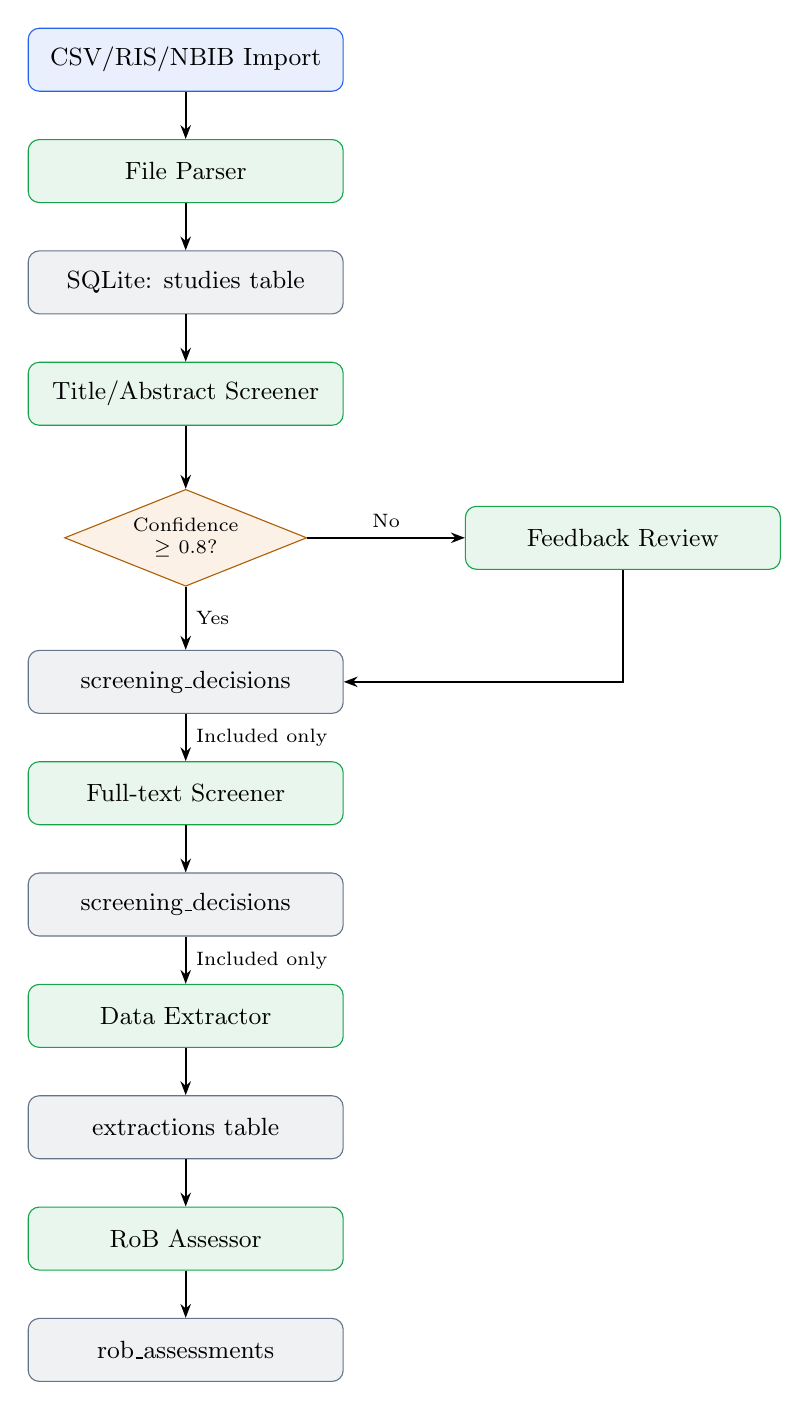
\begin{tikzpicture}[
  node distance=0.5cm,
  box/.style={draw, rounded corners=4pt, minimum width=4cm, minimum height=0.8cm, align=center, font=\small},
  data/.style={box, fill=primary!10, draw=primary},
  process/.style={box, fill=success!10, draw=success},
  decision/.style={diamond, draw=warning!80!black, fill=warning!10, aspect=2.5, inner sep=2pt, font=\scriptsize, align=center},
  store/.style={box, fill=secondary!10, draw=secondary},
  arr/.style={-{Stealth[length=5pt]}, thick},
]

\node[data] (import) {CSV/RIS/NBIB Import};
\node[process, below=0.6cm of import] (parse) {File Parser};
\node[store, below=0.6cm of parse] (studies) {SQLite: studies table};
\node[process, below=0.6cm of studies] (ta) {Title/Abstract Screener};
\node[decision, below=0.8cm of ta] (d1) {Confidence\\$\geq$ 0.8?};
\node[process, right=2cm of d1] (feedback) {Feedback Review};
\node[store, below=0.8cm of d1] (ta_dec) {screening\_decisions};
\node[process, below=0.6cm of ta_dec] (ft) {Full-text Screener};
\node[store, below=0.6cm of ft] (ft_dec) {screening\_decisions};
\node[process, below=0.6cm of ft_dec] (extract) {Data Extractor};
\node[store, below=0.6cm of extract] (extr) {extractions table};
\node[process, below=0.6cm of extr] (rob) {RoB Assessor};
\node[store, below=0.6cm of rob] (rob_r) {rob\_assessments};

\draw[arr] (import) -- (parse);
\draw[arr] (parse) -- (studies);
\draw[arr] (studies) -- (ta);
\draw[arr] (ta) -- (d1);
\draw[arr] (d1) -- node[right, font=\scriptsize]{Yes} (ta_dec);
\draw[arr] (d1) -- node[above, font=\scriptsize]{No} (feedback);
\draw[arr] (feedback) |- (ta_dec);
\draw[arr] (ta_dec) -- node[right, font=\scriptsize]{Included only} (ft);
\draw[arr] (ft) -- (ft_dec);
\draw[arr] (ft_dec) -- node[right, font=\scriptsize]{Included only} (extract);
\draw[arr] (extract) -- (extr);
\draw[arr] (extr) -- (rob);
\draw[arr] (rob) -- (rob_r);

\end{tikzpicture}
\caption{Complete data flow from reference import to final assessment.}
\end{figure}

\subsection{LLM Request/Response Flow}

For every LLM-powered operation, the following flow occurs:

\begin{enumerate}[nosep]
  \item \textbf{Cost estimation}: \texttt{CostTracker.estimate\_cost()} checks budget
  \item \textbf{Prompt construction}: Operation-specific template filled with data
  \item \textbf{Rate limiting}: \texttt{TokenBucket.wait\_for\_capacity()} (OpenAI only)
  \item \textbf{API call}: \texttt{LLMClient.chat(messages, json\_mode=True)}
  \item \textbf{Retry}: On 429/5xx errors, exponential backoff up to 5 retries
  \item \textbf{Response parsing}: JSON extraction from LLM response
  \item \textbf{Cost recording}: \texttt{CostTracker.add\_cost()} with actual token counts
  \item \textbf{Audit logging}: \texttt{AuditLogger.log\_llm\_call()} with full prompt/response
  \item \textbf{Persistence}: \texttt{SessionManager.save\_*()} to SQLite
\end{enumerate}

% ══════════════════════════════════════════════════════════════════════
\section{Database Schema}
% ══════════════════════════════════════════════════════════════════════

\begin{table}[H]
\centering\small
\begin{tabular}{lp{8cm}}
\toprule
\textbf{Table} & \textbf{Key Columns} \\
\midrule
\texttt{project} & id, name, research\_question, review\_type, criteria (JSON), llm\_provider, llm\_model, budget\_limit, current\_phase, timestamps \\
\texttt{studies} & id, pmid, doi, title, abstract, authors, year, journal, pdf\_path, pdf\_text, source\_database, created\_at \\
\texttt{screening\_decisions} & id, study\_id, phase, decision, reason, reason\_category, confidence, criteria\_evaluation (JSON), feedback fields \\
\texttt{extractions} & id, study\_id, field\_name, value, is\_not\_reported, source\_quote, notes, source, confidence \\
\texttt{extraction\_fields} & id, field\_name, description, field\_type, category, required, display\_order, options (JSON) \\
\texttt{audit\_log} & id, operation\_type, prompt, response, input\_tokens, output\_tokens, cost, model, study\_id, decision, timestamp \\
\texttt{cost\_tracking} & id, operation\_type, input\_tokens, output\_tokens, cost, model, timestamp \\
\texttt{rob\_assessments} & id, study\_id, tool\_type, overall\_judgment, overall\_rationale, ai\_cost, assessment\_status, assessor\_info \\
\texttt{rob\_judgments} & id, assessment\_id, domain\_name, judgment\_level, rationale, signaling\_responses (JSON), ai\_confidence \\
\texttt{rob\_templates} & id, tool\_type, name, description, domains (JSON), version \\
\texttt{rob\_settings} & id, project\_id, enabled\_tools (JSON), dual\_review, auto\_detect, batch\_queue (JSON) \\
\texttt{search\_strategies} & id, project\_id, pico\_analysis (JSON), concept\_blocks (JSON), database strategies (JSON) \\
\texttt{parsed\_references} & id, project\_id, source\_file, title, abstract, authors, year, journal, doi, pmid, dedup\_status \\
\bottomrule
\end{tabular}
\caption{Complete SQLite database schema (13 tables).}
\end{table}

% ══════════════════════════════════════════════════════════════════════
\section{Cost Model}
% ══════════════════════════════════════════════════════════════════════

\subsection{Per-Operation Cost Estimates}

\begin{table}[H]
\centering
\begin{tabular}{lrrr}
\toprule
\textbf{Operation} & \textbf{Input Tokens} & \textbf{Output Tokens} & \textbf{Cost (GPT-4o-mini)} \\
\midrule
Title/Abstract Screening & 500 & 100 & \$0.0001 \\
Full-text Screening & 4,000 & 300 & \$0.0008 \\
Data Extraction & 3,000 & 500 & \$0.0008 \\
Risk of Bias & 3,000 & 400 & \$0.0007 \\
Criteria Generation & 200 & 500 & \$0.0003 \\
PICO Analysis & 200 & 400 & \$0.0003 \\
PubMed Generation & 500 & 600 & \$0.0004 \\
\bottomrule
\end{tabular}
\caption{Per-study cost estimates at GPT-4o-mini pricing.}
\end{table}

\subsection{Example: 100-Study Review}

\begin{table}[H]
\centering
\begin{tabular}{lrr}
\toprule
\textbf{Phase} & \textbf{Studies} & \textbf{Estimated Cost} \\
\midrule
Title/Abstract Screening & 100 & \$0.01 \\
Full-text Screening (50 included) & 50 & \$0.04 \\
Data Extraction & 50 & \$0.04 \\
Risk of Bias Assessment & 50 & \$0.04 \\
\midrule
\textbf{Total (GPT-4o-mini)} & & \textbf{\$0.13} \\
\textbf{Total (GPT-4o)} & & \textbf{\$4.25} \\
\textbf{Total (Claude Sonnet 4)} & & \textbf{\$2.55} \\
\bottomrule
\end{tabular}
\caption{Total cost scaling for a 100-study systematic review.}
\end{table}

% ══════════════════════════════════════════════════════════════════════
\section{Configuration Reference}
% ══════════════════════════════════════════════════════════════════════

\subsection{Application Settings (config/settings.py)}

\begin{lstlisting}[style=python, title=Default Configuration]
@dataclass
class LLMSettings:
    openai_api_key: Optional[str] = None
    openai_default_model: str = "gpt-4o"
    anthropic_api_key: Optional[str] = None
    anthropic_default_model: str = "claude-sonnet-4-20250514"
    default_temperature: float = 0.3
    default_max_tokens: int = 1000

@dataclass
class ScreeningSettings:
    low_confidence_threshold: float = 0.8
    auto_include_threshold: float = 0.95
    batch_size: int = 50
    max_retries: int = 3

@dataclass
class ExtractionSettings:
    max_text_chars: int = 50000
    ocr_enabled: bool = True
    ocr_dpi: int = 200

@dataclass
class StorageSettings:
    default_storage_path: str = "~/systematic_reviews"
    database_name: str = "project.db"
\end{lstlisting}

\subsection{Environment Variables}

\begin{table}[H]
\centering\small
\begin{tabular}{lp{6cm}l}
\toprule
\textbf{Variable} & \textbf{Description} & \textbf{Default} \\
\midrule
\texttt{OPENAI\_API\_KEY} & OpenAI API key & None \\
\texttt{ANTHROPIC\_API\_KEY} & Anthropic API key & None \\
\texttt{DEBUG} & Debug mode & false \\
\texttt{STORAGE\_PATH} & Custom storage directory & \texttt{\textasciitilde/systematic\_reviews} \\
\texttt{OPENAI\_TPM\_LIMIT} & Tokens per minute & 90000 \\
\texttt{SCREENING\_MAX\_ABSTRACT\_CHARS} & Abstract truncation & 2000 \\
\texttt{SCREENING\_MAX\_TITLE\_CHARS} & Title truncation & 300 \\
\bottomrule
\end{tabular}
\caption{Environment variable reference.}
\end{table}

% ══════════════════════════════════════════════════════════════════════
\section{Deployment}
% ══════════════════════════════════════════════════════════════════════

\subsection{Development Setup}

\textbf{Backend:}
\begin{lstlisting}[style=python, title=Backend Setup]
cd reviewpyper-react/backend
pip install -r requirements.txt
uvicorn main:app --reload --port 8000
# API docs: http://localhost:8000/docs
\end{lstlisting}

\textbf{Frontend:}
\begin{lstlisting}[style=python, title=Frontend Setup]
cd reviewpyper-react/frontend
npm install
npm run dev
# Opens: http://localhost:5173
\end{lstlisting}

\subsection{Production Build}

\begin{lstlisting}[style=python, title=Production Build]
# Frontend
cd frontend && npm run build
# Output: dist/ (38.8 KB CSS, 386 KB JS, 116 KB gzipped)

# Backend
uvicorn main:app --host 0.0.0.0 --port 8000 --workers 4
\end{lstlisting}

% ══════════════════════════════════════════════════════════════════════
\section{Complete API Endpoint Reference}
% ══════════════════════════════════════════════════════════════════════

\begin{longtable}{llp{4cm}p{3cm}}
\toprule
\textbf{Method} & \textbf{Endpoint} & \textbf{Request Body} & \textbf{Response} \\
\midrule
\endfirsthead
\toprule
\textbf{Method} & \textbf{Endpoint} & \textbf{Request Body} & \textbf{Response} \\
\midrule
\endhead
\bottomrule
\endfoot

GET & /api/health & -- & \{status: ok\} \\
\midrule
\multicolumn{4}{l}{\textbf{Projects}} \\
POST & /api/projects & ProjectCreate & ProjectDetail \\
GET & /api/projects & -- & ProjectSummary[] \\
GET & /api/projects/\{id\} & -- & ProjectDetail \\
DELETE & /api/projects/\{id\} & -- & 204 \\
\midrule
\multicolumn{4}{l}{\textbf{LLM}} \\
POST & /api/llm/configure & LLMConfigureRequest & LLMConfigureResponse \\
GET & /api/llm/models & -- & ModelInfo[] \\
POST & /api/llm/test & LLMTestRequest & LLMTestResponse \\
GET & /api/llm/costs & -- & CostSummary \\
\midrule
\multicolumn{4}{l}{\textbf{Screening}} \\
POST & .../criteria & CriteriaRequest & CriteriaOut \\
GET & .../criteria & -- & CriteriaOut \\
POST & .../references/upload & multipart/form-data & \{count\} \\
GET & .../references & ?page\&page\_size & ReferenceListResponse \\
POST & .../screening/title-abstract & -- & ScreeningStatusResponse \\
GET & .../screening/ta/status & ?task\_id & ScreeningStatusResponse \\
POST & .../screening/fulltext & FulltextScreeningRequest & ScreeningStatusResponse \\
GET & .../screening/results & ?phase\&decision\&min\_conf & ScreeningResultsResponse \\
POST & .../screening/feedback & FeedbackRequest & \{updated\} \\
\midrule
\multicolumn{4}{l}{\textbf{Extraction}} \\
POST & .../extraction/fields/recommend & FieldRecommendRequest & ExtractionFieldOut[] \\
POST & .../extraction/fields & FieldSaveRequest & ExtractionFieldOut[] \\
GET & .../extraction/fields & -- & ExtractionFieldOut[] \\
POST & .../extraction/run & -- & ExtractionStatusResponse \\
GET & .../extraction/results & -- & ExtractionResultsResponse \\
\midrule
\multicolumn{4}{l}{\textbf{Risk of Bias}} \\
GET & /api/rob/templates & -- & RoBTemplateInfo[] \\
POST & .../rob/assess & RoBAssessRequest & RoBStatusResponse \\
GET & .../rob/results & -- & RoBResultsResponse \\
\midrule
\multicolumn{4}{l}{\textbf{Search Strategy}} \\
POST & .../search/pico & PICORequest & PICOResponse \\
POST & .../search/generate & GenerateRequest & GenerateResponse \\
POST & .../search/translate & TranslateRequest & TranslateResponse \\
POST & .../search/validate & ValidateRequest & ValidateResponse \\
\midrule
\multicolumn{4}{l}{\textbf{Export}} \\
GET & .../export/csv & ?phase & text/csv \\
GET & .../export/prisma & -- & PRISMACountsOut \\

\end{longtable}

% ══════════════════════════════════════════════════════════════════════
\section{Component Dependency Graph}
% ══════════════════════════════════════════════════════════════════════

\begin{figure}[H]
\centering
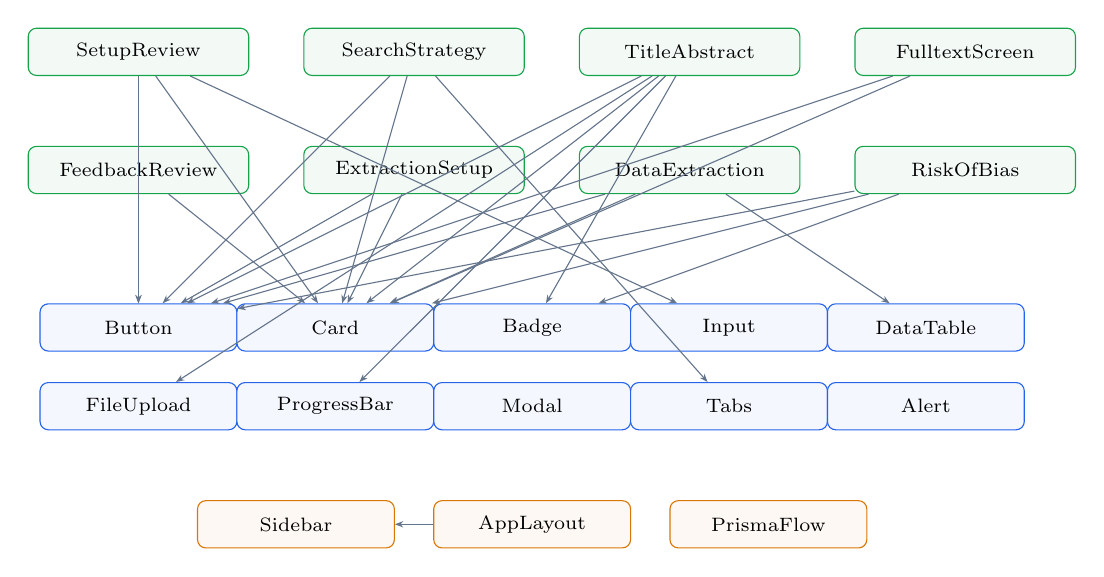
\begin{tikzpicture}[
  node distance=0.4cm and 1.2cm,
  comp/.style={draw=primary, fill=primary!5, rounded corners=3pt, minimum width=2.5cm, minimum height=0.6cm, align=center, font=\scriptsize},
  page/.style={draw=success, fill=success!5, rounded corners=3pt, minimum width=2.8cm, minimum height=0.6cm, align=center, font=\scriptsize},
  arr/.style={-{Stealth[length=3pt]}, thin, secondary},
]

% Pages
\node[page] (setup) at (0,0) {SetupReview};
\node[page] (search) at (3.5,0) {SearchStrategy};
\node[page] (screen) at (7,0) {TitleAbstract};
\node[page] (ft) at (10.5,0) {FulltextScreen};
\node[page] (fb) at (0,-1.5) {FeedbackReview};
\node[page] (es) at (3.5,-1.5) {ExtractionSetup};
\node[page] (de) at (7,-1.5) {DataExtraction};
\node[page] (rs) at (10.5,-1.5) {RiskOfBias};

% Shared components
\node[comp] (btn) at (0,-3.5) {Button};
\node[comp] (card) at (2.5,-3.5) {Card};
\node[comp] (badge) at (5,-3.5) {Badge};
\node[comp] (input) at (7.5,-3.5) {Input};
\node[comp] (table) at (10,-3.5) {DataTable};
\node[comp] (upload) at (0,-4.5) {FileUpload};
\node[comp] (prog) at (2.5,-4.5) {ProgressBar};
\node[comp] (modal) at (5,-4.5) {Modal};
\node[comp] (tabs) at (7.5,-4.5) {Tabs};
\node[comp] (alert) at (10,-4.5) {Alert};

% Layout
\node[comp, draw=warning, fill=warning!5] (layout) at (5,-6) {AppLayout};
\node[comp, draw=warning, fill=warning!5] (sidebar) at (2,-6) {Sidebar};
\node[comp, draw=warning, fill=warning!5] (prisma) at (8,-6) {PrismaFlow};

% Representative arrows
\foreach \p in {setup, search, screen, ft, fb, es, de, rs} {
  \draw[arr] (\p) -- (btn);
  \draw[arr] (\p) -- (card);
}

\draw[arr] (screen) -- (upload);
\draw[arr] (screen) -- (prog);
\draw[arr] (screen) -- (badge);
\draw[arr] (search) -- (tabs);
\draw[arr] (rs) -- (badge);
\draw[arr] (de) -- (table);
\draw[arr] (setup) -- (input);

\draw[arr] (layout) -- (sidebar);

\end{tikzpicture}
\caption{Frontend component dependency graph (simplified).}
\end{figure}

% ══════════════════════════════════════════════════════════════════════
\section{Summary Statistics}
% ══════════════════════════════════════════════════════════════════════

\begin{table}[H]
\centering
\begin{tabular}{lr}
\toprule
\textbf{Metric} & \textbf{Count} \\
\midrule
\multicolumn{2}{l}{\textbf{Original Core (Python)}} \\
Core modules & 9 \\
Python source files & 40+ \\
Pydantic models & 30+ \\
LLM prompt templates & 16 \\
RoB tool templates & 5 \\
SQLite tables & 13 \\
\midrule
\multicolumn{2}{l}{\textbf{FastAPI Backend}} \\
API routers & 7 \\
REST endpoints & 30 \\
Pydantic request/response models & 35+ \\
Background task workers & 3 \\
\midrule
\multicolumn{2}{l}{\textbf{React Frontend}} \\
Page components & 9 \\
Reusable UI components & 11 \\
Layout components & 2 \\
Special components & 1 (PrismaFlow) \\
TypeScript interfaces & 15 \\
React Query hooks & 30+ \\
API service methods & 30+ \\
Routes & 10 \\
\midrule
\multicolumn{2}{l}{\textbf{Build Output}} \\
CSS bundle & 38.8 KB \\
JS bundle & 386 KB (116 KB gzipped) \\
\bottomrule
\end{tabular}
\caption{Project statistics.}
\end{table}

\end{document}
